

%\begin{table}
%	\caption{Declare Mining for  over the BPI 2012 Challenge. }
%	\centering
%	\resizebox{\textwidth}{!}
%	{\begin{tabular}{lr|rr|rr}
%			\toprule
%			\multirow{2}{*}{\textit{Template}+ModelSize} & \multirow{2}{*}{\textit{Log Size}} & \multicolumn{4}{c}{Query Time \textit{(ms)}} \\ 
%		&	& \textsf{SQLMiner} & \textsf{SQLMiner+TraceInfo} & \textbf{KnoBAB+MaxSat}& \textbf{KnoBAB+Supp}\\
%			\midrule
%			\textit{Response+25} & 10 & $1.46\cdot 10^0$ & $\color{red}1.70\cdot 10^2$ & $\mathbf{9.08}\cdot \mathbf{10}^\mathbf{-1}$ & $9.21\cdot 10^{-1}$\\
%			\textit{Response+25} & 100 & $6.09\cdot 10^0$ & $\color{red}7.86\cdot 10^2$ & $ \mathbf{3.39}\cdot  \mathbf{10}^ \mathbf{0}$& $3.62\cdot 10^0$\\
%			\textit{Response+25} & 1\,000 & $6.53\cdot 10^1$ & $\color{red}4.58\cdot 10^4$ & $ \mathbf{2.97}\cdot  \mathbf{10}^ \mathbf{1}$& $3.13\cdot 10^1$\\
%			\textit{Response+25} & 10\,000 & $ \mathbf{2.39}\cdot  \mathbf{10}^ \mathbf{2}$ & $\color{red}4.84\cdot 10^6$ & $\mathbf{3.02}\cdot \mathbf{10}^\mathbf{2}$& $3.08\cdot 10^2$\\
%			\bottomrule
%	\end{tabular}}
%\end{table}


\section{Experimental Analysis}\label{sec:exp}
These benchmarks were carried out on a Razer Blade Pro laptop with Intel Core i7-10875H CPU @ 2.30GHz (Max 5.10 GHz) (8 Cores 16 Logical Processors), 16GB DDR4 2933MHz RAM and 315GB free disk space.
\begin{figure}[!t]
	\centering
	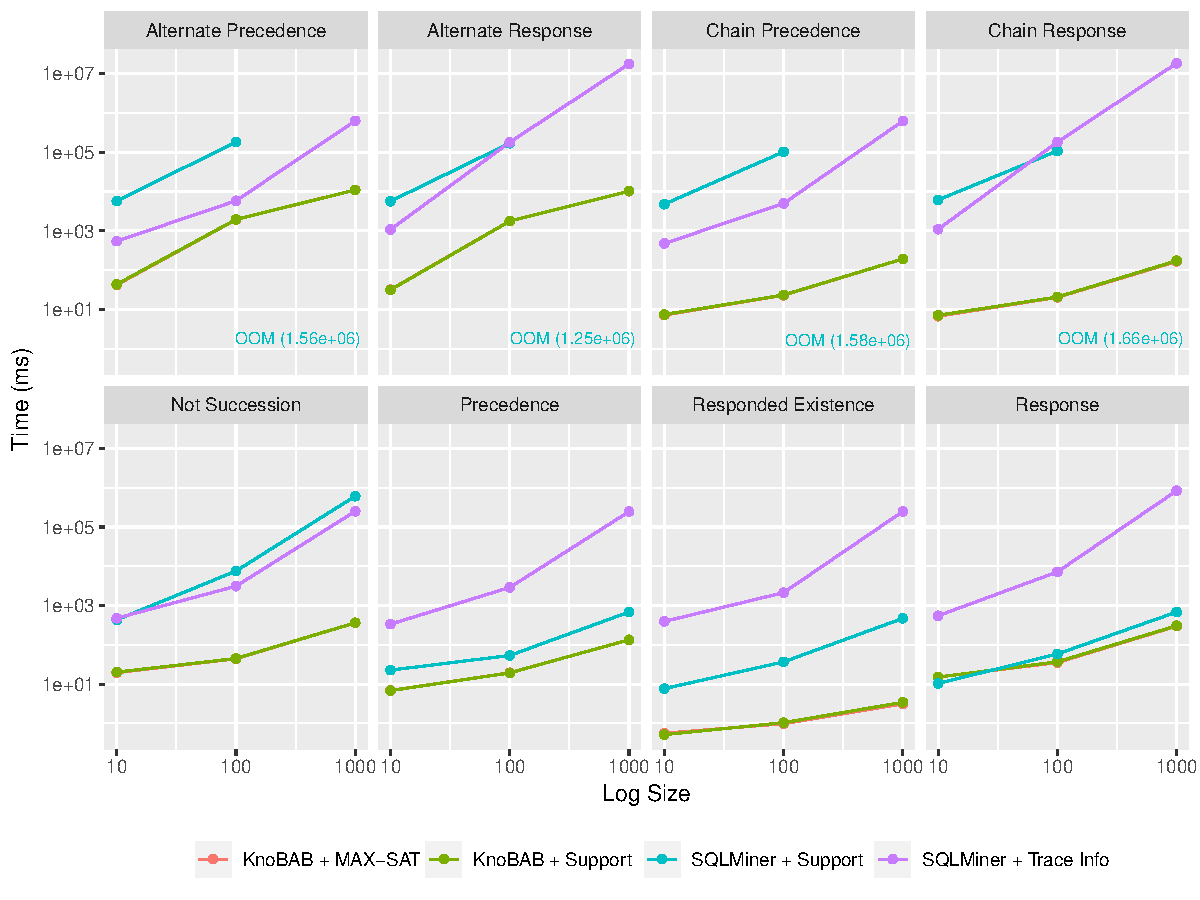
\includegraphics[width=.8\textwidth]{images/sqlminer_benchmark.pdf}
	\caption{KnoBAB vs SQLMiner Performance for Varying Model Size.}\label{fig:vsSQL}
\end{figure}

\subsection{SQLMiner}\label{ssec:sqlmin}

\textbf{PostgreSQL 13.5}  (\figurename~\ref{fig:vsSQL})

\begin{figure}[!t]
	\centering
	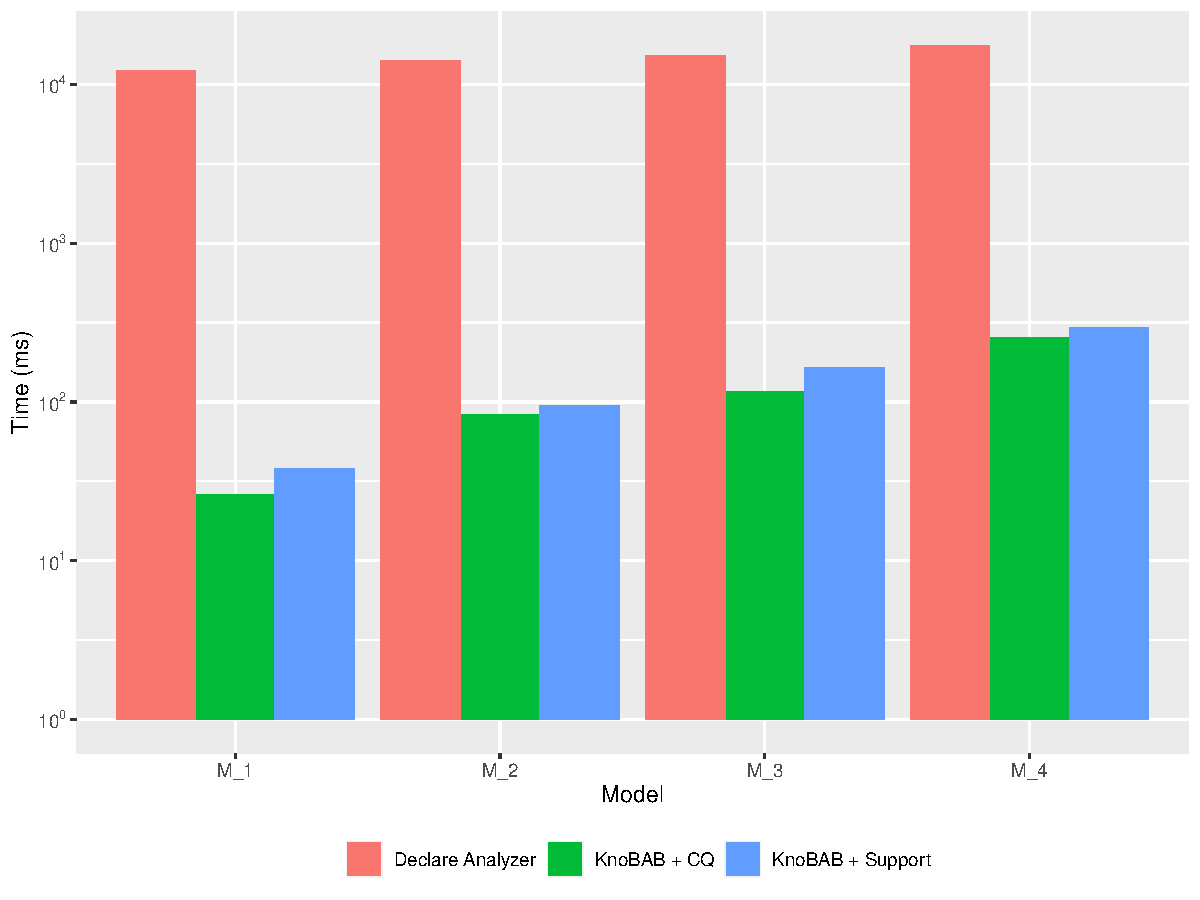
\includegraphics[width=.8\textwidth]{images/burattin_benchmark.pdf}
	\caption{KnoBAB vs Declare Analyzer Performance for Different Models.}\label{fig:vsSQL}
\end{figure}

\subsection{Declare Analyzer}\label{ssec:declan}

\begin{table}[!t]
	\caption{Declare Models with their Respective Clauses}
	\resizebox{\textwidth}{!}{
		\begin{tabular}{l|l}
			Model & Queries \\
			\toprule
			\multirow{2}{*}{$M\_1=$} & $q_{1}:= \DeclareClause{Response}{A\_SUBMITTED}{\textbf{true}}{A\_ACCEPTED}{\textbf{true}}$ \\ & $q_{2}:= \DeclareClause{Response}{A\_SUBMITTED}{\texttt{AMOUNT\_REQ} \geq 10^3}{A\_ACCEPTED}{\textbf{true}}$ \\&
			$q_{3}:= \DeclareClause{Response}{A\_SUBMITTED}{\texttt{AMOUNT\_REQ} < 10^3}{A\_ACCEPTED}{\textbf{true}}$ \\&
			$q_{4}:= q_{1} \textrm{ where } \texttt{A\_SUBMITTED.org:resource}=\texttt{A\_ACCEPTED.org:resource}$ \\&
			$q_{5}:= q_{1} \textrm{ where } \texttt{A\_SUBMITTED.org:resource}\neq\texttt{A\_ACCEPTED.org:resource}$ \\
			\toprule
			\multirow{2}{*}{$M\_2=M_1+$} & $q_{6}:= \DeclareClause{Response}{W\_Completeren aanvraag}{\textbf{true}}{W\_Valideren aanvraag}{\textbf{true}}$ \\ &
			$q_{7}:= \DeclareClause{Response}{W\_Completeren aanvraag}{\textbf{true}}{O\_CANCELLED}{\textbf{true}}$ \\&
			$q_{8}:= q_{6} \textrm{ where } \texttt{A\_SUBMITTED.org:resource}\neq\texttt{A\_ACCEPTED.org:resource}$ \\&
			$q_{9}:= \DeclareClause{Response}{W\_Valideren aanvraag}{\texttt{AMOUNT\_REQ} = 5 \cdot 10^3}{O\_CANCELLED}{\textbf{true}} $ \\&
			$q_{10}:= q_{9} \textrm{ where } \texttt{A\_SUBMITTED.org:resource}=\texttt{A\_ACCEPTED.org:resource}$ \\
			\toprule
			\multirow{2}{*}{$M\_3=M_2+$} & $q_{11}:= \DeclareClause{Response}{O\_SELECTED}{\textbf{true}}{O\_CANCELLED}{\textbf{true}}$ \\&
			$q_{12}:= q_{11} \textrm{ where } \texttt{A\_SUBMITTED.org:resource}=\texttt{A\_ACCEPTED.org:resource}$ \\&
			$q_{13}:= \DeclareClause{Response}{O\_SELECTED}{\texttt{AMOUNT\_REQ} < 8 \cdot 10^3}{O\_CANCELLED}{\textbf{true}}$ \\&
			$q_{14}:= q_{13} \textrm{ where } \texttt{A\_SUBMITTED.org:resource}=\texttt{A\_ACCEPTED.org:resource}$ \\&
			$q_{15}:= \DeclareClause{Response}{O\_SELECTED}{\texttt{AMOUNT\_REQ} > 10^3}{O\_CANCELLED}{\textbf{true}}$ \\
			\toprule
			\multirow{2}{*}{$M\_4=M_3+$} & $q_{16}:= \DeclareClause{Response}{A\_PARTLYSUBMITTED}{\textbf{true}}{A\_DECLINED}{\textbf{true}}$ \\&
			$q_{17}:= q_{16} \textrm{ where } \texttt{A\_SUBMITTED.org:resource}=\texttt{A\_ACCEPTED.org:resource}$ \\&
			$q_{18}:= \DeclareClause{Response}{A\_PARTLYSUBMITTED}{\texttt{AMOUNT\_REQ} > 2 \cdot 10^4}{A\_DECLINED}{\textbf{true}}$ \\&
			$q_{19}:= \DeclareClause{Response}{A\_PARTLYSUBMITTED}{\texttt{AMOUNT\_REQ} > 2 \cdot 10^4}{A\_CANCELLED}{\textbf{true}}$ \\&
			$q_{20}:= q_{18} \textrm{ where } \texttt{A\_SUBMITTED.org:resource}=\texttt{A\_ACCEPTED.org:resource}$ \\
	\end{tabular}}
\end{table}


The benefits from the custom query plan are most obvious in the process mining stage, where a log consisting of potentially thousands of traces is tested against all combinations of clauses. However, computational gains can also be evidenced when the same querying approach is adapted to a runtime scenario, where we are querying only 1 trace against an existing model (which requires much less computation as a whole).

For $\mathcal{C}$ Declare clauses, where $\mathcal{N}$ is the data loading cost, implementations without a KB suffer, resulting in $\mathcal{O(C \cdot N)}$ complexity. With a KB, data loading is necessary only once, enhancing the complexity to $\mathcal{O(C + N)}$.

However these are computationally bottlenecked to the efficiency of these systems themselves, regardless of the optimality of the conformance checking.

\RevDel{SQL miner, due to the query structure, requires vast amounts of secondary memory for temporary caching of query computation, {much less than KnoBAB requires}.}